
Un entorno de visualización de eventos de \ROOT ~creado como parte del proyecto \textbf{ALICE} es \textbf{EVE} (\textbf{E}vent \textbf{V}isualization \textbf{E}nvironment), el mismo proporciona un marco de aplicación para la construcción de programas de visualización de eventos, está construido sobre la infraestructura GUI, GL y GED, el mismo ofrece las siguientes características principales:

\begin{itemize_f}
	\item[-] Clases base para la representación de objetos visuales que se pueden presentar en vistas de árbol de lista, editores de objetos y renderizados a 	través de OpenGL (TEveElement y subclases).
	\item[-] Clase de administrador de aplicaciones TEveManager para la gestión de nivel superior de elementos, componentes GUI, geometrías y eventos.
	\item[-] Clases para la presentación de geometrías TGeo completas (TEveGeoNode y TEveGeoTopNode), así como de geometrías simplificadas mediante extracción de datos de forma (TEveGeoShape).
\end{itemize_f}

\begin{figure}[ht!]
    \centering
    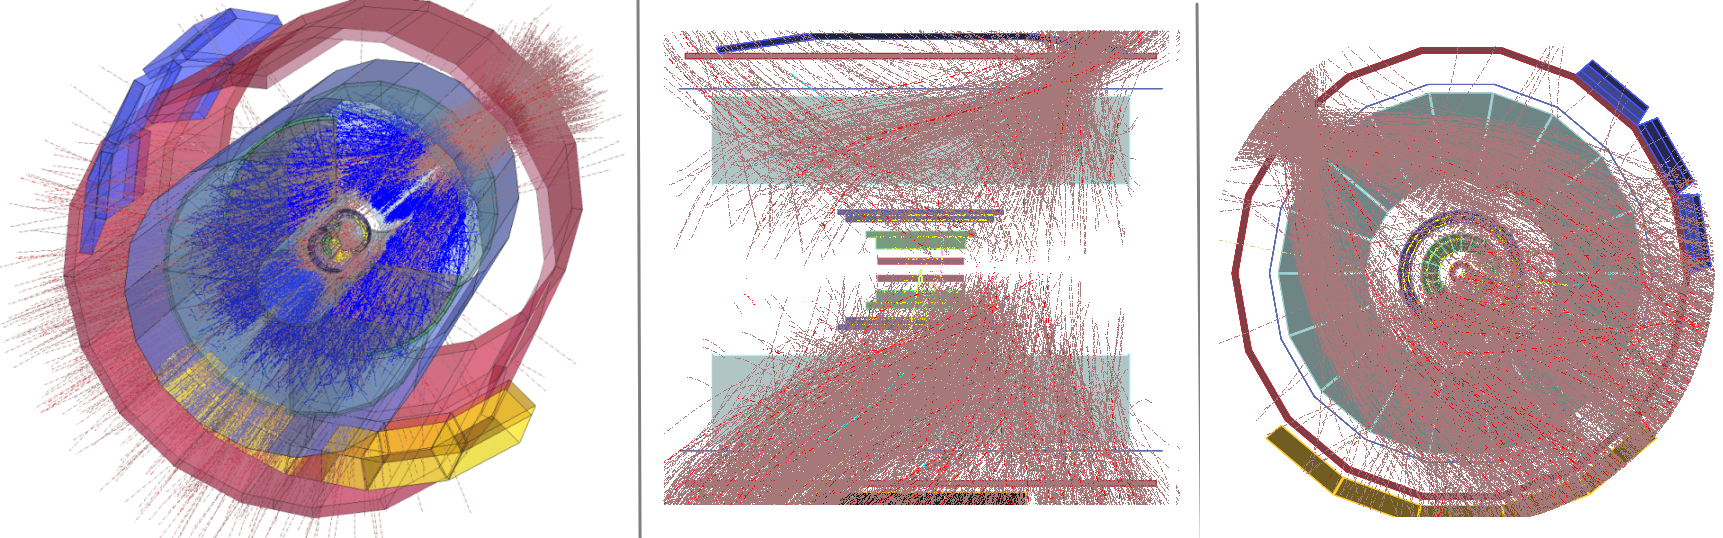
\includegraphics[width=0.84\textwidth]{Analisis_y_Resultados/imagenes/Eve_rand-alieve2.png}
    \caption{Diagrama de flujo de la investigación.}
    \label{fig:Eve_rand-alieve}
\end{figure}
Para su implementación se hace necesario seguir los pasos simplificados mostrados en la guía \url{https://cp3.irmp.ucl.ac.be/projects/delphes/wiki/WorkBook/EventDisplay} y hacer uso de los comandos:

\begin{minipage}{0.9\linewidth}
\vspace{5pt}%margen superior de minipage
{\small 
\begin{verbatim}
	make display
	root -l examples/EventDisplay.C'("cards/delphes_card_CMS.tcl","delphes_output.root")'
\end{verbatim}}
\end{minipage}